\subsubsection{Temple University} 
\paragraph*{Commercial Triple-GEM Detectors}\mbox{}\\
Temple University was able to achieve several goals that were set for this funding cycle. 
Last summer two commercial triple-GEM detectors were built, one using Kapton rings as the spacers between the GEM layers and another using more traditional G10 spacer grids. Upon completion of the two triple-GEM detectors, they were inserted into the cosmic ray test bench where both detectors drew about twice as much current as the STAR FGT triple-GEM detectors, and exhibited excessive sparking. This sparking ultimately led to both detectors failing and becoming unusable. After opening the detectors and inspecting the layers, the effects of excessive sparking were clear, as can be seen in fig.~\ref{fig:spark}. It was hypothesized that the sparking was a result of shorts originating in the HV connector pads on the GEM foils in each layer. Each GEM foil is segmented into nine HV sectors on one side, while the other side is unsegmented. Each of the nine HV sectors connects to three HV pads located at the top of the GEM foil. Additionally, there are three pads which connect to the unsegmented side of the GEM foil, as shown in fig.~\ref{fig:EICFGT}. The HV pin connections are then made to a HV pad position that is associated with one of the three triple-GEM layers, \emph{e.g.} the middle GEM foil layer has HV pins connected to the HV pads in the center of the three pads for each sector. In the initial two triple-GEM detectors built, the unused HV pads for each GEM foil layer were left in tack with the thinking that the pins passing through the unused HV pads would be isolated from them since they are not physically touching the HV pads. However this turned out not to be the case and was found to be the cause of the shorts in the initial commercial triple-GEM detectors. This was verified during the building of the third commercial triple-GEM detector. After stretching and gluing all foils to their respective frames, the triple-GEM stack was assembled by simply stacking the various layers without glue. We then tested the detector for shorts amongst the HV pins, where we were able to generate shorts with minor movements of the HV pins. The stack was then disassembled and all unused HV pads on each GEM foil were cut away. The detector stack was reassembled and tested again for shorts. With the excess HV pads removed we were not able to detect any shorts. Gluing the stack of the third commercial GEM detector and inserting it into the cosmic ray stand, we now see the same current being pulled as that STAR FGT triple-GEM detectors pull. This suggests that the shorting issue that plagued the first two triple-GEM detectors is now solved.      

Now that the shorting issue has been resolved we are ready to begin the characterization of the triple-GEM detector. Figure~\ref{fig:EICGFTcosmic} shows initial reconstructed cosmic ray hits.
There is enough material remaining to assemble a fourth commercial triple-GEM detector. The GEM, readout, and HV foils for this detector have now been stretched and glued to their respective frames. The assembly of the GEM stack was delayed until we saw how the third triple-GEM detector performed, in case we needed to correct any unforeseen issues.

\begin{figure}
\center
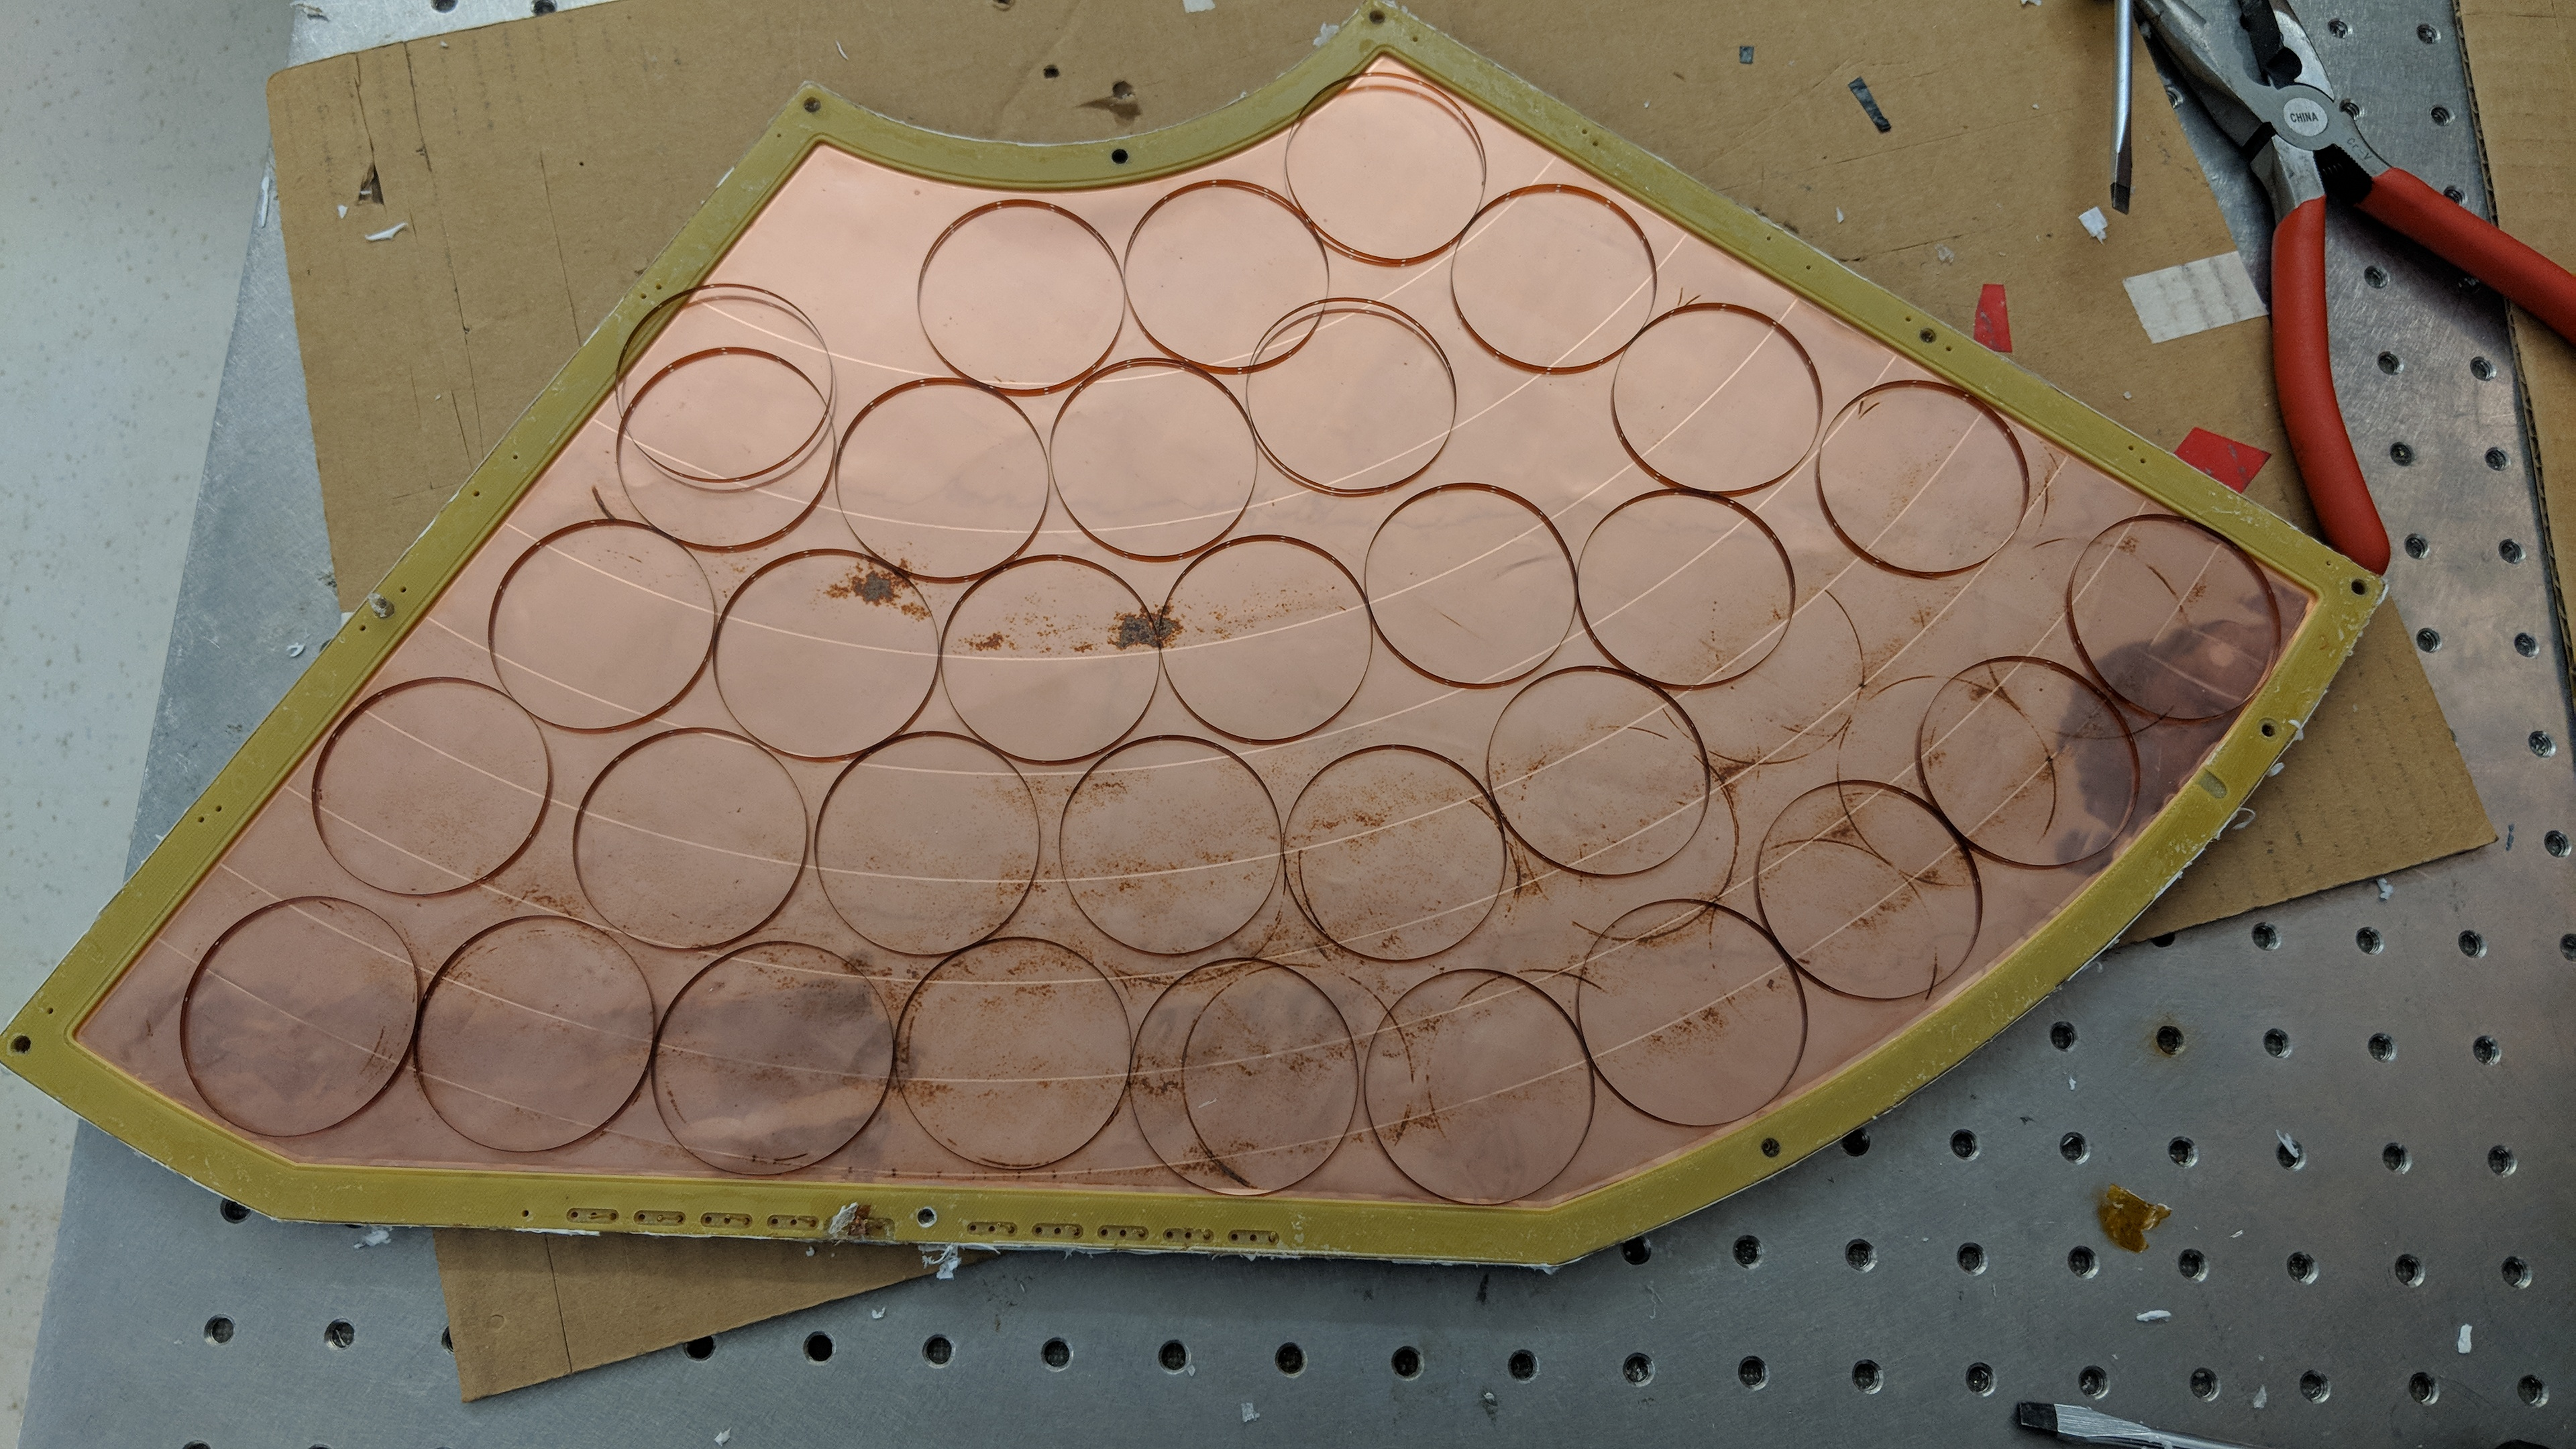
\includegraphics[width=\columnwidth]{TU_plots/GEM-spark.jpg}
\caption{\label{fig:spark}Damage to a GEM layer in the first commercial triple-GEM detector caused by excessive sparking resulting from electrical shorts.}
\end{figure}


\begin{figure}
\center
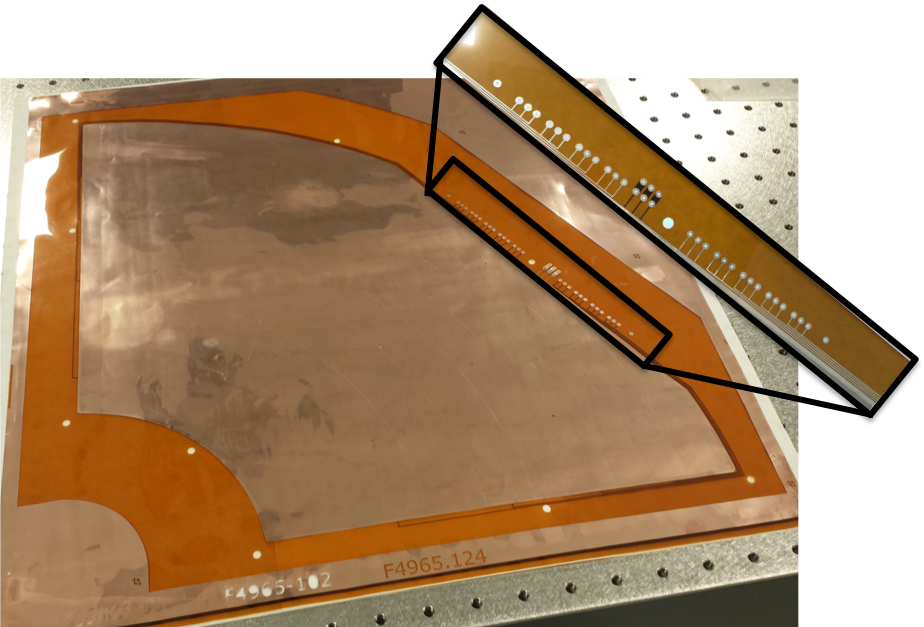
\includegraphics[width=\columnwidth]{TU_plots/GEM-HVPad.png}
\caption{\label{fig:EICFGT} Commercial GEM foil HV sectors and connection pads.}
\end{figure}

\begin{figure}
\center
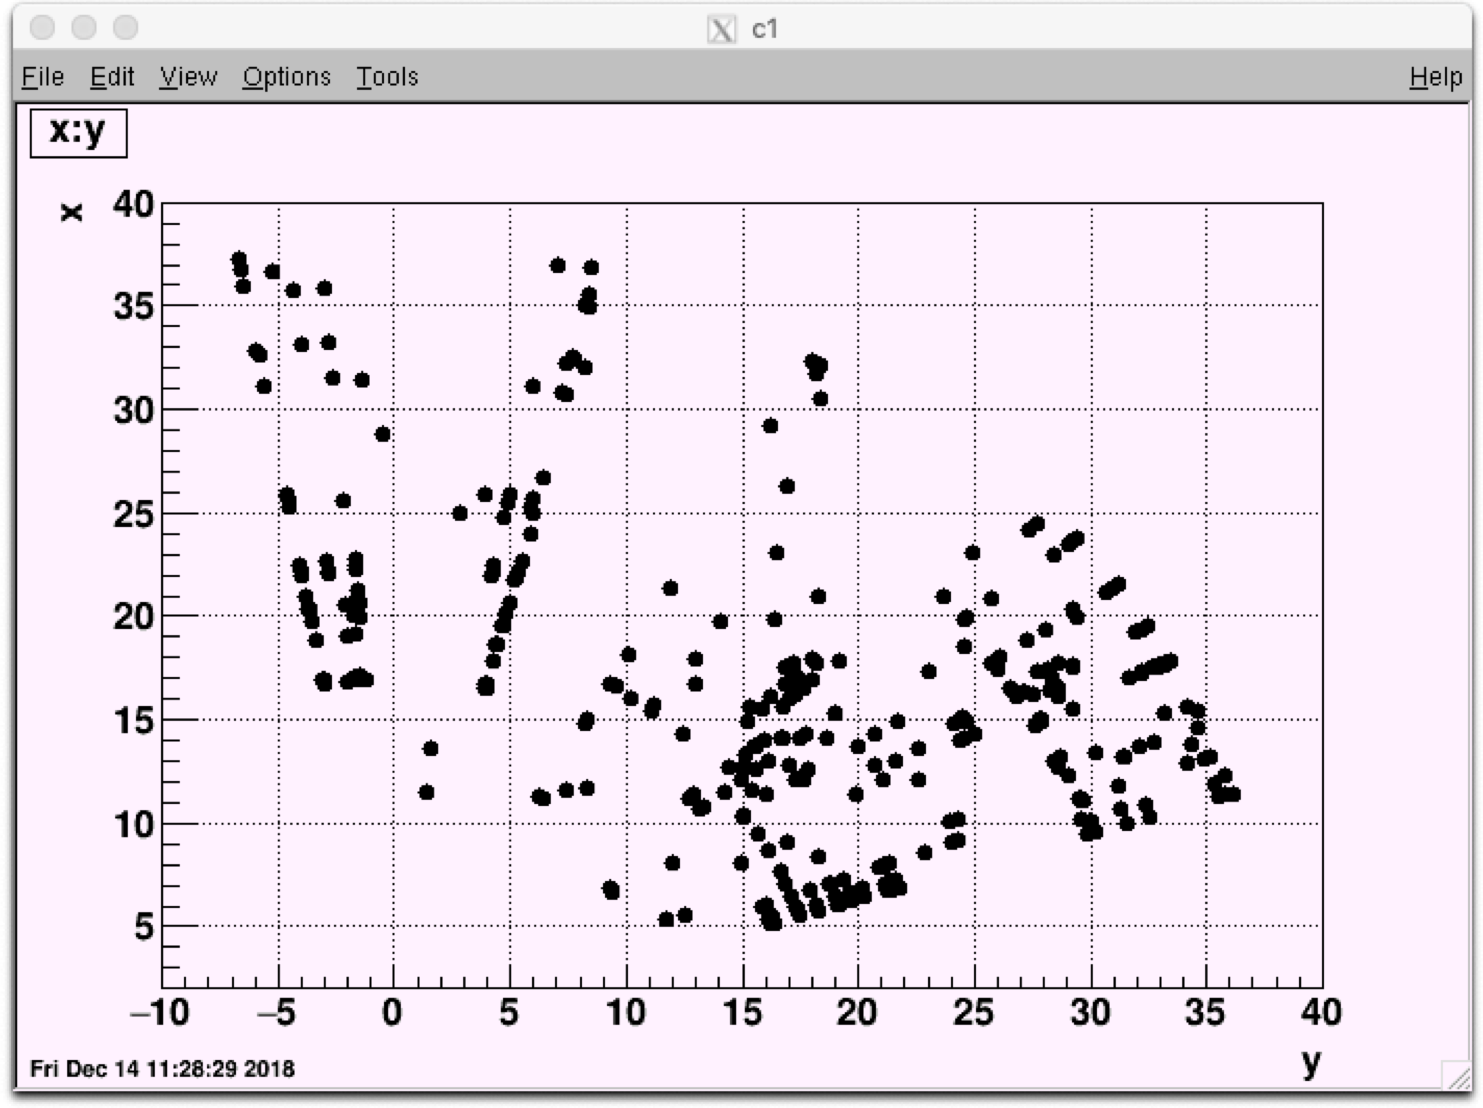
\includegraphics[width=\columnwidth]{TU_plots/Cosmic.png}
\caption{\label{fig:EICGFTcosmic}Commercial triple-GEM detector showing reconstructed X-Y hit of cosmic ray events.}
\end{figure}

\paragraph*{MPGD $\mu$TPC Simulation}\mbox{}\\
In addition to the hardware work, we are also working on some simulations. The initial machinery needed to produce a MPGD detector in $\mu$TPC mode has now been implemented. This machinery allows one to create a barrel geometry with a specified dead material radiation length and drift gap filled with a particular gas. This machinery also allows one to simulate multiple hit points by defining sensitive barrel layers within the drift gap volume. The resolution parameters of the detector are also adjustable. For example one can specify the detectors radial and transverse resolutions, as well as its hit point resolution. This machinery has now been tested using some nominal settings and is currently being modified to reflect more realistic parameters and digitization.